\thispagestyle{empty}
\ThisULCornerWallPaper{1}{../files/img/header.png}

\pagenumbering{roman}
\setcounter{page}{0}
\vspace*{6cm}
\begin{center}
\setmainfont[Scale=6]{Lato Bold}
FEniCS 2021
\end{center}
\begin{center}
\setmainfont[Scale=4]{Lato Bold}
22--26 March 2021
\end{center}

\vspace{8cm}

\begin{center}
\setmainfont[Scale=2]{Lato Bold}
Editors
\end{center}
\begin{center}
\setmainfont[Scale=1.3]{Lato}
Igor Baratta
\end{center}
\begin{center}
\setmainfont[Scale=1.3]{Lato}
J{\o}rgen S.~Dokken
\end{center}
\begin{center}
\setmainfont[Scale=1.3]{Lato}
Chris Richardson
\end{center}
\begin{center}
\setmainfont[Scale=1.3]{Lato}
Matthew W.~Scroggs
\end{center}


\tableofcontents


\chapter*{Introduction}
\pagenumbering{arabic}
\setcounter{page}{1}
\addcontentsline{toc}{chapter}{Introduction}

The FEniCS 2021 conference was held online in March 2021, using a combination of Zoom and Gather Town.
This document collects the abstracts and slides for the talks presented at FEniCS 2021.

The following picture was taking during the Gather Town evening session on Thursday 25 March.

\begin{center}
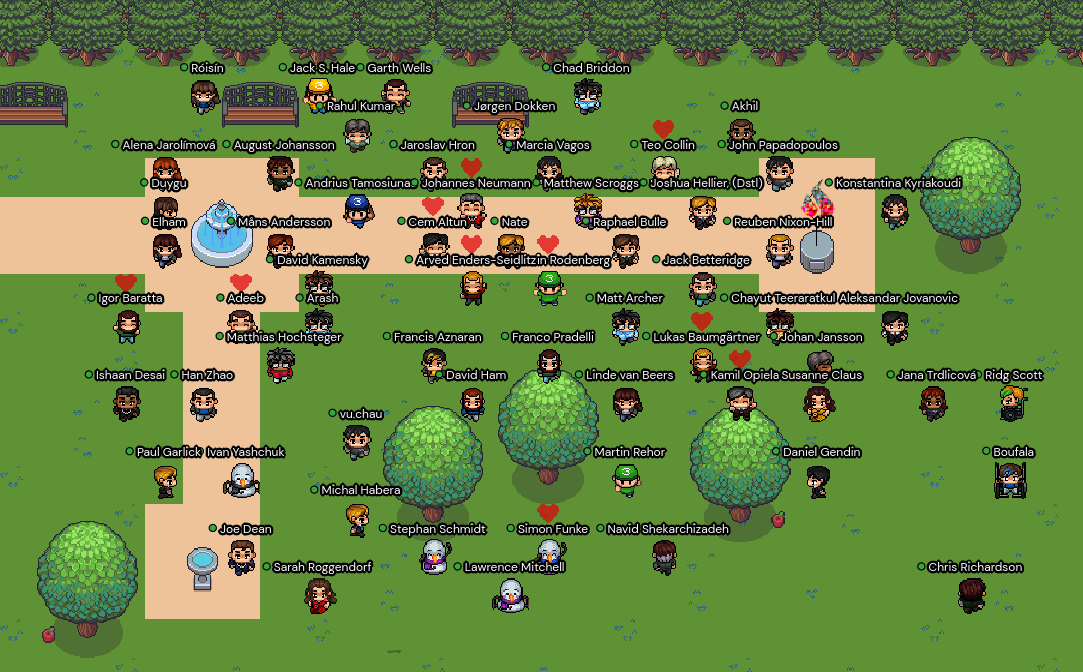
\includegraphics[width=0.9\textwidth]{../files/img/small-photo.png}
\end{center}

\section*{Prizes}

Three prizes were given at FEniCS 2021. These were awarded to:
\begin{itemize}
\item Best talk by a PhD student or undergraduate: Rémi Delaporte-Mathurin
\item Best talk by a PhD student or undergraduate (runner up): India Marsden
\item Best talk by a postdoc: Marc Hirschvogel
\end{itemize}

\noindent The prizes were kindly provided by Rafinex.
